\documentclass{article}\usepackage[]{graphicx}\usepackage[]{color}
%% maxwidth is the original width if it is less than linewidth
%% otherwise use linewidth (to make sure the graphics do not exceed the margin)
\makeatletter
\def\maxwidth{ %
  \ifdim\Gin@nat@width>\linewidth
    \linewidth
  \else
    \Gin@nat@width
  \fi
}
\makeatother

\definecolor{fgcolor}{rgb}{0.345, 0.345, 0.345}
\newcommand{\hlnum}[1]{\textcolor[rgb]{0.686,0.059,0.569}{#1}}%
\newcommand{\hlstr}[1]{\textcolor[rgb]{0.192,0.494,0.8}{#1}}%
\newcommand{\hlcom}[1]{\textcolor[rgb]{0.678,0.584,0.686}{\textit{#1}}}%
\newcommand{\hlopt}[1]{\textcolor[rgb]{0,0,0}{#1}}%
\newcommand{\hlstd}[1]{\textcolor[rgb]{0.345,0.345,0.345}{#1}}%
\newcommand{\hlkwa}[1]{\textcolor[rgb]{0.161,0.373,0.58}{\textbf{#1}}}%
\newcommand{\hlkwb}[1]{\textcolor[rgb]{0.69,0.353,0.396}{#1}}%
\newcommand{\hlkwc}[1]{\textcolor[rgb]{0.333,0.667,0.333}{#1}}%
\newcommand{\hlkwd}[1]{\textcolor[rgb]{0.737,0.353,0.396}{\textbf{#1}}}%

\usepackage{framed}
\makeatletter
\newenvironment{kframe}{%
 \def\at@end@of@kframe{}%
 \ifinner\ifhmode%
  \def\at@end@of@kframe{\end{minipage}}%
  \begin{minipage}{\columnwidth}%
 \fi\fi%
 \def\FrameCommand##1{\hskip\@totalleftmargin \hskip-\fboxsep
 \colorbox{shadecolor}{##1}\hskip-\fboxsep
     % There is no \\@totalrightmargin, so:
     \hskip-\linewidth \hskip-\@totalleftmargin \hskip\columnwidth}%
 \MakeFramed {\advance\hsize-\width
   \@totalleftmargin\z@ \linewidth\hsize
   \@setminipage}}%
 {\par\unskip\endMakeFramed%
 \at@end@of@kframe}
\makeatother

\definecolor{shadecolor}{rgb}{.97, .97, .97}
\definecolor{messagecolor}{rgb}{0, 0, 0}
\definecolor{warningcolor}{rgb}{1, 0, 1}
\definecolor{errorcolor}{rgb}{1, 0, 0}
\newenvironment{knitrout}{}{} % an empty environment to be redefined in TeX

\usepackage{alltt}
\usepackage{graphicx}
\usepackage[english]{babel}
\usepackage{csquotes}
\usepackage{url}
\usepackage{scrextend}

\usepackage{mathptmx} 

\usepackage[backend=bibtex]{biblatex}
\addbibresource{pepr-pub.bib}


\IfFileExists{upquote.sty}{\usepackage{upquote}}{}
\begin{document}
\title{
        Pipelines for Evaluating Prokaryotic References \\ 
        \large{Supplemental Material}\\
        Candidate Reference Material Sequencing and Genome Assembly
}
\maketitle

\section{Material Development}
Sequencing data for the NIST candidate reference material RM8376, genomic DNA from \emph{Staphylococcus aureus} strain NRS100 isolate COL (Biosample SAMN02854573) was selected as a model system to demonstrate how PEPR is used to characterize a microbial genomic material.  The strain was isolated from a clinical sample by Children's National Hospital (Biosample SAMN02700075). The genomic material represents a large homogeneous batch of extracted DNA, with 1500 vials each with $3\mu g$.  The extracted DNA was prepared from single colony of the initial culture stab was incubated overnight at 37°C on an agar plate and a single colony was used to inoculate a new plate. One colony from the new plate was grown in 20 mL Luria-Bertani (LB) broth at 37°C. The culture was used to inoculate 15 X 150 mm plates which were incubated at 37°C for 16 hours. DNA was isolated by lysing the bacteria in lysis solution containing NaCl, Tris, EDTA and lysostaphin ($25\mu g/ml$) and SDS. Proteinase K and RNase A were used to treat protein and RNA. Ammonium acetate was used to remove protein. DNA was recovered by isopropanol precipitation. DNA was washed with 70\% alcohol, drained, and dissolved in TE buffer (Tris 10 mM, EDTA 0.1 mM, pH8.0).

\section{Sequencing Experimental Design}
The \emph{S. aureus} candidate reference materials were sequenced using three orthogonal sequencing platforms: Pacific Biosciences RSII (PacBio)\footnote{\label{pacbio}Pacific Biosciences of California Inc.\url{http://www.pacificbiosciences.com/} 1380 Willow Rd. Menlo Park, CA 94025 USA}, Ion Torrent PGM \footnote{\label{pgm}Life Technologies Corp., \url{http://www.iontorrent.com/} 7000 Shoreline Court \# 201, South San Francisco, CA 94080 USA}, and Illumina MiSeq \footnote{\label{illumina}Illumina Inc., \url{http://www.illumina.com/} 5200 Illumina Way San Diego, CA 92122 USA}. For PacBio sequencing, the sequencing library was prepared using DNA Template Prep Kit 3.0 with pooled DNA from three randomly sampled vials of the candidate reference material RM8376. The resulting library was sequenced with the P6-C4 chemistry.  
For the Ion Torrent PGM \footref{pgm} and Illumina MiSeq \footref{illumina} sequencing, eight vials were randomly sampled from the lot of 1500 vials. For MiSeq, two technical replicate libraries were prepared for each of the eight vials using the Nextera DNA Sample Prep Kit\footref{illumina}; samples were barcoded using the Nextera Index Kit and sequenced using the MiSeq 600 cycle Reagent kit v3 for 2 X 300 bp reads.  The 16 libraries were pooled and sequenced in a single run.  Single barcoded 400 bp Ion Torrent PGM libraries were prepared for each of the eight vials using the Ion Xpress Plus kit \footref{pgm}.  The vials were barcoded using the IonXpress Kit\footref{illumina}, sequencing template was prepared using the Ion PGM Template OT2 400 kit and the IonPGM400 kit was used for sequencing on a 318C chip. The raw sequence data is archived in the Genbank Sequence Read Archive (http://www.ncbi.nlm.nih.gov/sra), see Table 1 of main paper for accession numbers.  A genome map was obtained for the candidate reference material from optical mapping data generated using the Argus Optical Mapping System\footnote{\label{opgen}OpGen Inc. \url{http://opgen.com} 708 Quince Orchard Road Gaithersburg, MD 20878 USA}. Agarose plugs generated from the same culture stock as that used to generate the DNA reference material were used for optical mapping measurement.  Restriction enzyme NcoI was used for the restriction digest. These steps occured prior to our PEPR pipeline.

\section{\emph{S. aureus} Reference Assembly}
PacBio long read data were used to generate a \emph{de novo} genome assembly for use in the Genome Evaluation Pipeline. PacBio Reads were assembled using SMRTAnalysis software version 2.3 \footref{pacbio} to apply the HGAP assembly algorithm \cite{Koren2013}.  To identify potential errors in the assembly, an \emph{in silico} digest of assembly was compared the genome map obtained from the optical mapping data using OpGen MapSolver software\footref{opgen}. The \emph{de novo} assembly was supported by Optical mapping data (Fig. \ref{fig:opgenCompFig}). The plasmid is too small for OpGen optical mapping technology, and therefore the plasmid assembly was not validated with the optical mapping data. 

\begin{figure}
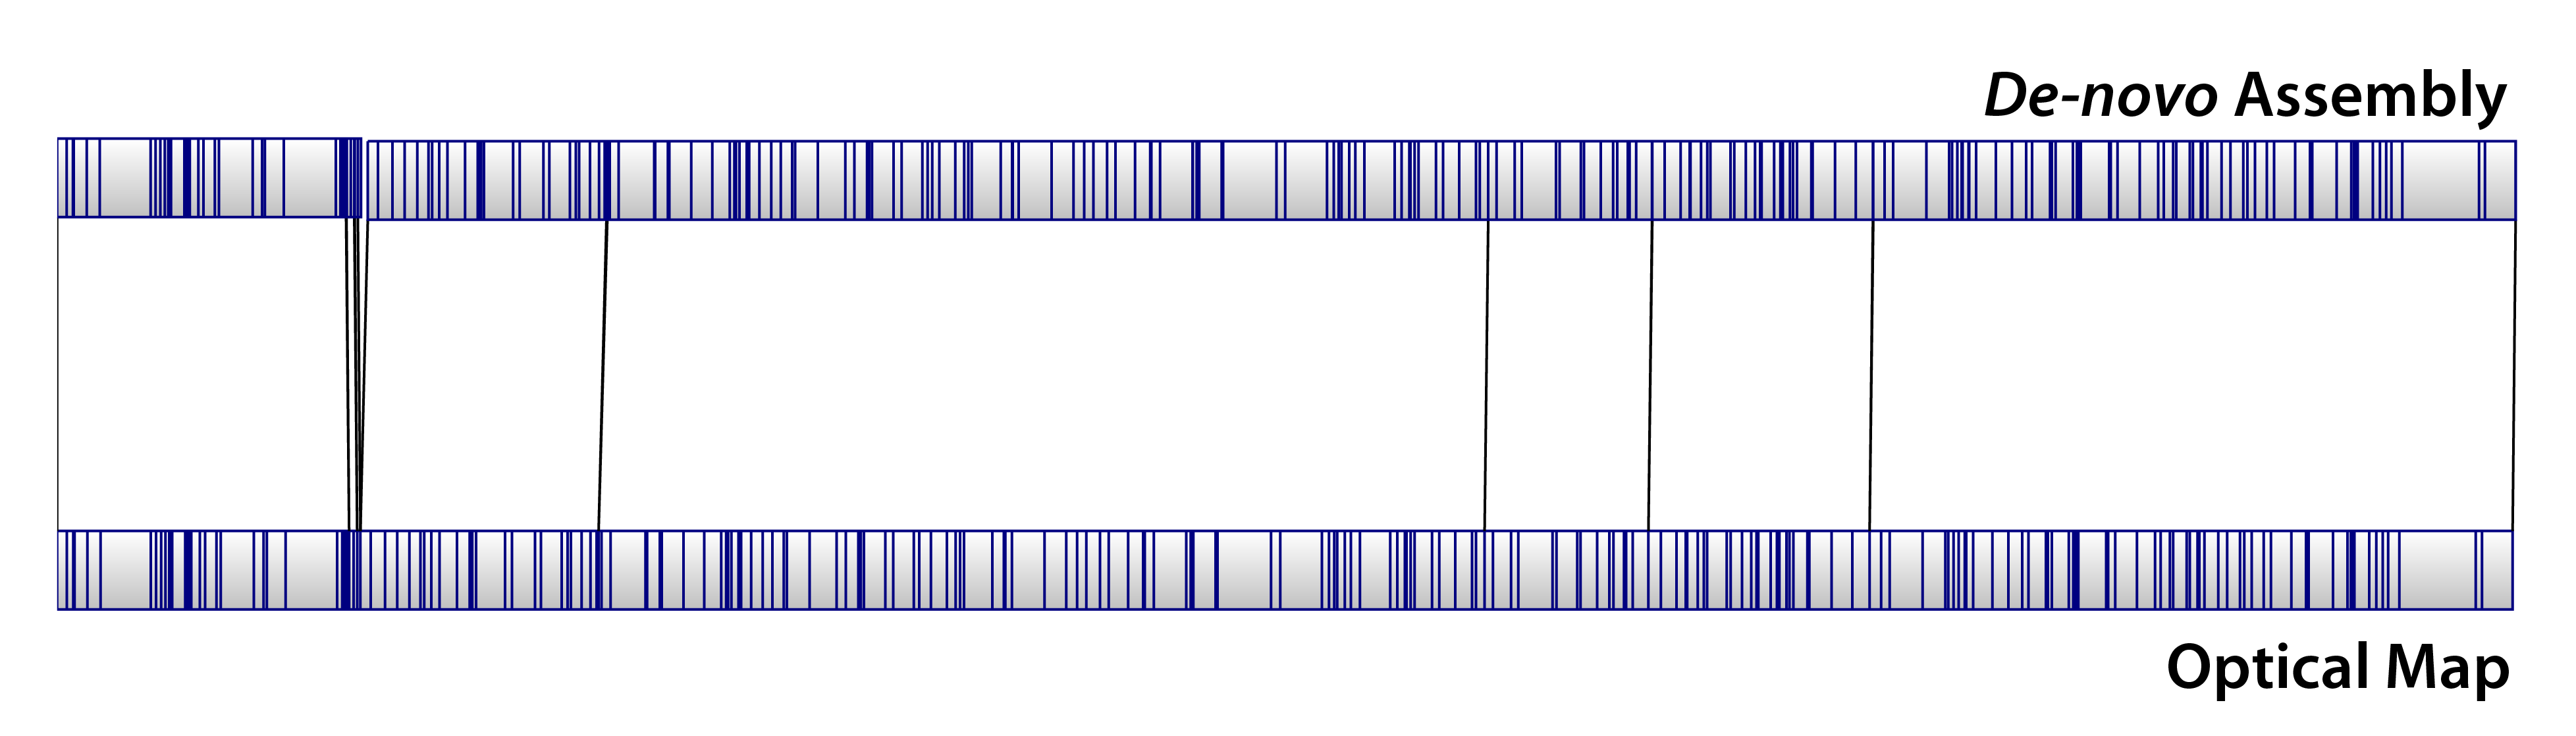
\includegraphics[width=\textwidth]{opgen_assembly_comparison.png}
\label{fig:opgenCompFig}
\caption{Comparison of optical map data to genome assembly. Alignment of \emph{in-silico} genome map generated from the PacBio HGAP assembly to the OpGen optical map.  Blue bars in map represent NocI restriction sites, black lines indicate co-linear regions.}
\end{figure}

\printbibliography
\end{document}
